\documentclass{beamer}
\input{macros_beamer.tex}
\begin{document}
\begin{frame}
\title{《丰富的图形世界》综合质量检测卷答案}
一、BDBBB  CDDDA
二、109.圆锥,长方体\ 
12.线,点,线,面,体

13.长方体,三棱柱,9,17,10

14.6 \ 15.24 \ 16.6 \ 17.72  \ 18.6、7或8

19.(1)---c (2)---d (3)---a (4)---b

20.解:(1)这个棱柱共有10个顶点,15条棱。

(2)这个棱柱有7个面,它的侧面积为\[2\times4\times5=40(\mathrm{cm}^2)\]

21.B(1);C(1,2,3);D(4);E(3,4,5)
\end{frame}


\begin{frame}
23.解:依题意知$x,y,z$的对面分别是0,4,1,

所以$x+0=y+4=z+1=5$,

解得$x=5,y=1,z=4$.

所以$x+y+z=10$.
\end{frame}


\begin{frame}
24.
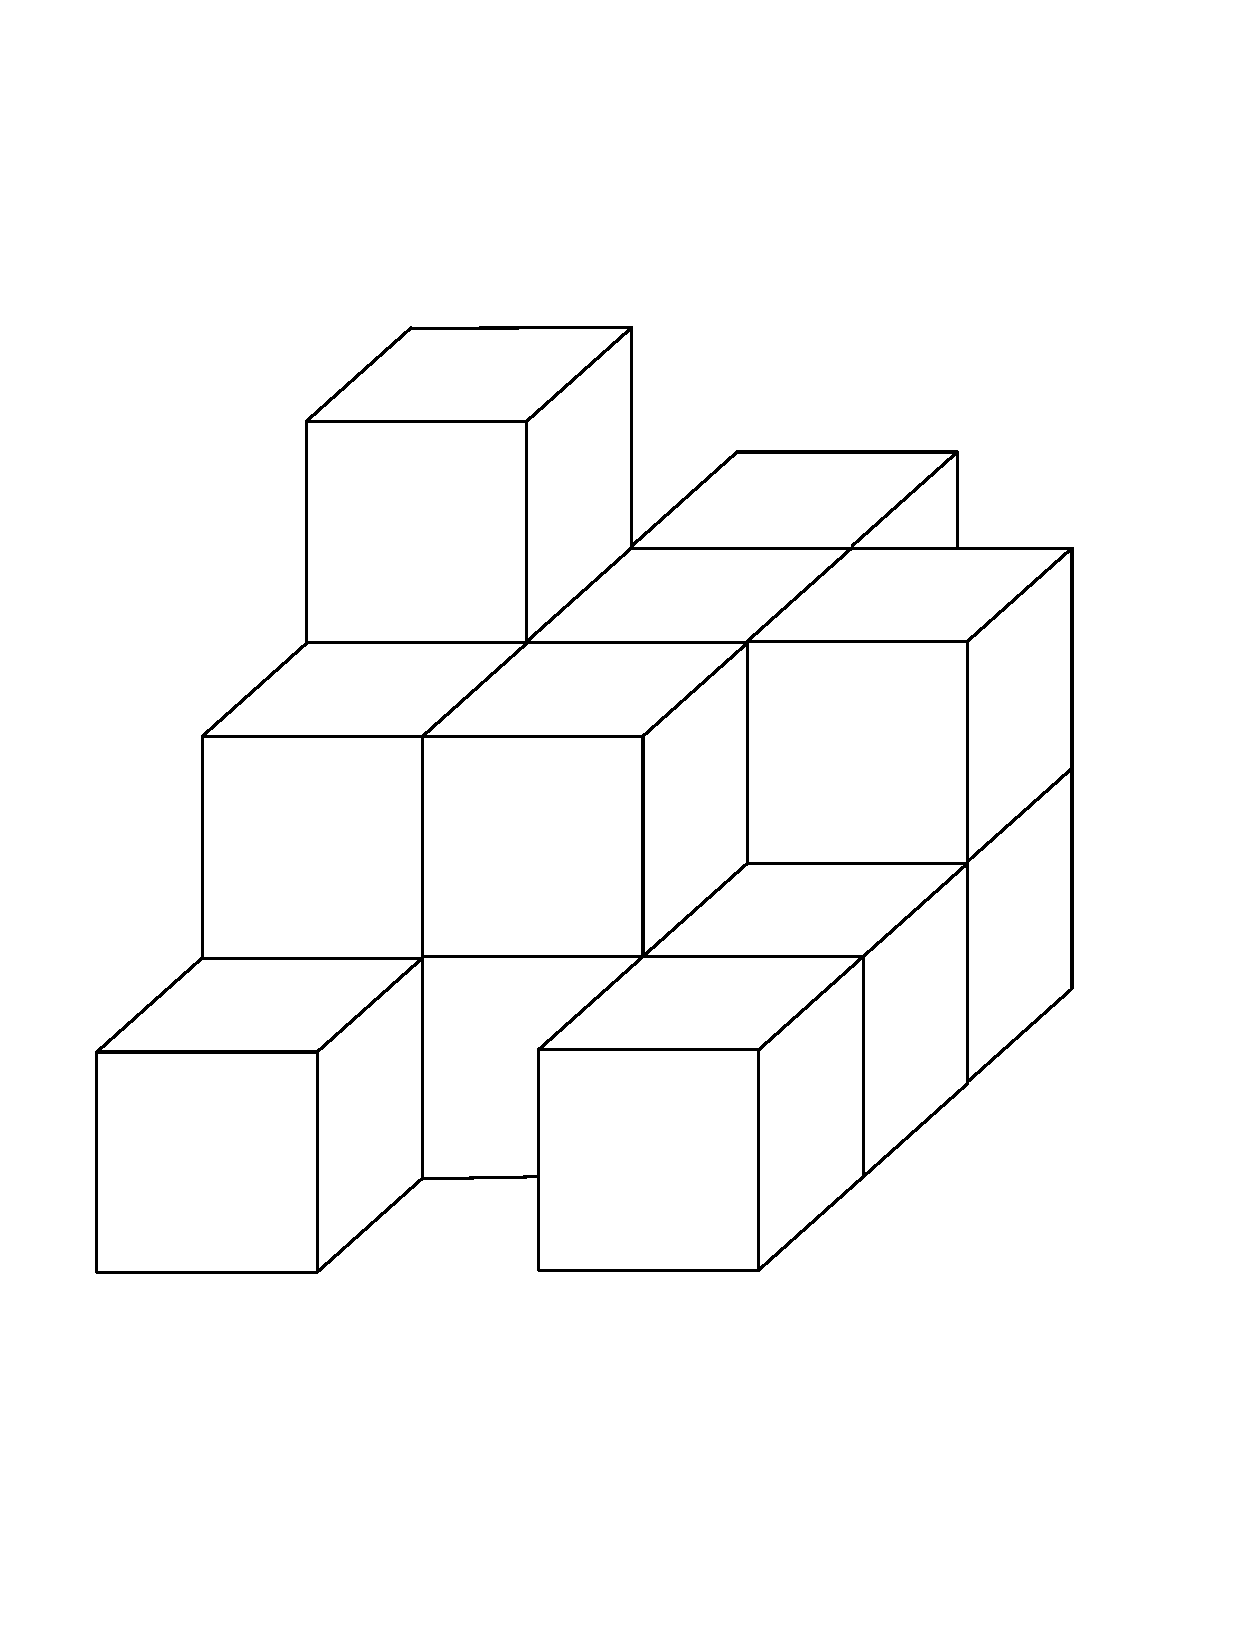
\includegraphics[width=3in]{200cm.pdf}
\end{frame}

\end{document}
